\documentclass[12pt,a4paper]{article}
\usepackage[utf8]{vietnam}
\usepackage{amsmath}
\usepackage{graphicx}
\usepackage{tikz}
\usepackage{tikz-cd}
\usepackage{booktabs}
\usepackage{multirow}
\usepackage[left=2cm,right=2cm,top=2cm,bottom=2cm]{geometry}

% Định nghĩa các màu và style cho đồ thị
\tikzset{
    vertex/.style={circle,draw,minimum size=1cm},
    edge/.style={->,>=stealth},
    loop/.style={min distance=5mm,in=120,out=60}
}

\title{Phân tích Mạng xã hội - Bài tập nhóm}
\author{Phân tích các mạng xã hội}
\date{\today}

\begin{document}

\maketitle
\tableofcontents
\newpage

\section{Bài tập 1: Phân tích mạng học tập}

\subsection{Yêu cầu}
\begin{enumerate}
\item Tính mật độ mạng
\item Xác định các số đo trung tâm
\item Tính số đo gom cụm cho mỗi sinh viên
\item Nhận xét vai trò của Em trong nhóm
\end{enumerate}

\subsection{Giải}

\subsubsection{Biểu diễn đồ thị}
\begin{center}
\begin{tikzpicture}
\node[circle,draw] (A) at (0,2) {An};
\node[circle,draw] (B) at (2,2) {Bình};
\node[circle,draw] (E) at (1,1) {Em};
\node[circle,draw] (D) at (0,0) {Dung};
\node[circle,draw] (C) at (2,0) {Cường};

\draw (A) -- (B);
\draw (A) -- (E);
\draw (B) -- (E);
\draw (D) -- (E);
\draw (C) -- (E);
\draw (D) -- (C);
\draw (A) -- (D);
\draw (B) -- (C);
\end{tikzpicture}
\end{center}

\subsubsection{Tính mật độ mạng}
Mật độ của mạng được tính theo công thức:
\[ D = \frac{2L}{N(N-1)} \]

Trong đó:
\begin{itemize}
\item L: số cạnh trong đồ thị = 8 (đếm trực tiếp từ đồ thị)
\item N: số đỉnh trong đồ thị = 5 (An, Bình, Em, Dung, Cường)
\end{itemize}

Thay số:
\[ D = \frac{2 \times 8}{5 \times 4} = \frac{16}{20} = 0.8 \]

Nhận xét: Mật độ mạng 0.8 (80\%) cho thấy đây là mạng kết nối khá chặt chẽ.

\subsubsection{Các số đo trung tâm}
\paragraph{a. Degree Centrality}
\[ C_D(v) = \frac{deg(v)}{N-1} \]

\begin{itemize}
\item Em: $C_D(Em) = \frac{4}{4} = 1$
\item Các thành viên khác: $C_D(v) = \frac{3}{4} = 0.750$
\end{itemize}

\paragraph{b. Closeness Centrality}
\[ C_C(v) = \frac{N-1}{\sum_{t \in V\setminus\{v\}} d(v,t)} \]

\begin{itemize}
\item Em: $C_C(Em) = \frac{4}{1+1+1+1} = 1.000$ (khoảng cách trung bình ngắn nhất)
\item Các thành viên khác: $C_C(v) =\frac{4}{1+1+2+1} = 0.800$
\end{itemize}

\paragraph{c. Betweenness Centrality}
\[ C_B(v) = \frac{\sum_{s \neq v \neq t} \frac{\sigma_{st}(v)}{\sigma_{st}}}{(N-1)(N-2)} \]

\begin{itemize}
\item Em: $C_B(Em) = \frac{2}{3}\times\frac{2}{4\times 3} = 0.111$ (vai trò trung gian quan trọng nhất)
\item Các thành viên khác: $C_B(v) = \frac{1}{3}\times\frac{2}{4\times 3} = 0.056$
\end{itemize}

\subsubsection{Số đo gom cụm}
\[ C_i = \frac{2|E(N_i)|}{k_i(k_i-1)} \]
Trong đó $|E(N_i)|$ là số cạnh giữa các láng giềng của i.

\begin{itemize}
\item Em: $C(Em) = \frac{2 \times 2}{2 \times 3} = 0.667$
\item Các thành viên khác: $C(v) = \frac{2 \times 2}{3 \times 2} = 0.667$
\item clustering Expectation: $\overline{C(v)} = 0.667$
\end{itemize}

\subsubsection{Phân tích vai trò của Em}
\begin{itemize}
\item \textbf{Vị trí trung tâm:}
    \begin{itemize}
    \item Degree cao nhất (1.000): kết nối trực tiếp với tất cả thành viên
    \item Closeness cao nhất (1.000): dễ dàng tiếp cận mọi thành viên
    \item Betweenness cao nhất (0.111): kiểm soát luồng thông tin
    \end{itemize}
\item \textbf{Tính kết nối:}
    \begin{itemize}
    \item Đóng vai trò cầu nối giữa các nhóm nhỏ trong mạng
    \item Tính kết nối ngang bằng với các bạn khác
    \end{itemize}
\item \textbf{Ảnh hưởng:}
    \begin{itemize}
    \item Là trung tâm trao đổi thông tin
    \item Có khả năng điều phối hoạt động nhóm
    \item Tạo môi trường học tập hiệu quả
    \end{itemize}
\end{itemize}

\section{Bài tập 2: Phân tích luồng thông tin trong tổ chức}

\subsection{Yêu cầu}
\begin{enumerate}
\item Tính mật độ mạng
\item Xác định các số đo trung tâm có hướng
\item Phân tích cấu trúc tổ chức
\item Đánh giá hiệu quả luồng thông tin
\end{enumerate}

\subsection{Giải Bài tập 2}
\subsubsection{Biểu diễn đồ thị}
\begin{center}
\begin{tikzpicture}[
    node distance=3cm,
    vertex/.style={circle,draw,minimum size=1cm},
    edge/.style={->,>=stealth,thick,bend left=20}
]
% Vẽ GD ở trên cùng
\node[vertex] (GD) at (0,2) {GD};

% Vẽ 4 phòng ban theo hình chữ nhật với khoảng cách rộng hơn
\node[vertex] (P1) at (-4.5,0) {P1};
\node[vertex] (P2) at (-1.5,0) {P2};
\node[vertex] (P3) at (1.5,0) {P3};
\node[vertex] (P4) at (4.5,0) {P4};

% Vẽ các mũi tên từ phòng ban lên GD với góc nghiêng khác nhau
\draw[edge] (P1) to[bend left=15] (GD);
\draw[edge] (P2) to[bend left=5] (GD);
\draw[edge] (P3) to[bend right=5] (GD);
\draw[edge] (P4) to[bend right=15] (GD);

% Vẽ các mũi tên giữa các phòng ban với đường cong
\draw[edge] (P1) to (P2);
\draw[edge] (P2) to (P3);
\draw[edge] (P3) to (P4);
\draw[edge, bend right=40] (P4) to (P1);

% Thêm chú thích
\node[below=0.3cm] at (P1) {Phòng 1};
\node[below=0.3cm] at (P2) {Phòng 2};
\node[below=0.3cm] at (P3) {Phòng 3};
\node[below=0.3cm] at (P4) {Phòng 4};
\node[above=0.3cm] at (GD) {Giám đốc};
\end{tikzpicture}
\end{center}

\subsubsection{Mật độ mạng}
Với đồ thị có hướng:
\[ D = \frac{L}{N(N-1)} = \frac{8}{5 \times 4} = 0.400 \]
\subsubsection{Bậc vào và ra:}
\begin{tabular}{|c|c|c|}
\hline
\textbf{Node} & \textbf{In-degree} & \textbf{Out-degree} \\
\hline
GD & 4 & 0 \\
P1 & 1 & 2 \\
P2 & 1 & 2 \\
P3 & 1 & 2 \\
P4 & 1 & 2 \\
\hline
\end{tabular}

\subsubsection{Các số đo trung tâm có hướng}
\paragraph{a. In/Out-Degree Centrality}
\begin{itemize}
\item GD: $C_{D,in}(GD) = 1.000$, $C_{D,out}(GD) = 0.000$
\item Các phòng ban: $C_{D,in}(P_i) = 0.250$, $C_{D,out}(P_i) = 0.500$
\end{itemize}

\paragraph{b. In/Out-Closeness Centrality}
\begin{itemize}
\item GD: $C_{in}(GD) = 0.000$, $C_{out}(GD) = 1.000$
\item Các phòng ban: $C_{in}(P_i) = 0.571$, $C_{out}(P_i) = 0.375$
\end{itemize}

\paragraph{c. Betweenness Centrality (chuẩn hóa)}
\begin{itemize}
\item GD: $C_B(GD) = 0.000$
\item Các phòng ban: $C_B(P_i) = 0.250$
\end{itemize}

\subsubsection{Phân tích cấu trúc tổ chức}
\begin{itemize}
\item \textbf{Cấu trúc phân cấp:}
    \begin{itemize}
    \item GD: Trung tâm tiếp nhận thông tin (in-degree cao nhất)
    \item Các phòng ban: Vị trí ngang hàng, trao đổi thông tin hai chiều
    \item Không có phản hồi trực tiếp từ GD xuống phòng ban
    \end{itemize}
\item \textbf{Hiệu quả luồng thông tin:}
    \begin{itemize}
    \item Ưu điểm:
        \begin{itemize}
        \item Thông tin tập trung về một đầu mối
        \item Trao đổi ngang cấp giữa các phòng ban
        \item Giảm nhiễu thông tin
        \end{itemize}
    \item Hạn chế:
        \begin{itemize}
        \item Thiếu kênh phản hồi từ GD
        \item Có thể chậm trong xử lý khủng hoảng
        \item Phụ thuộc vào hiệu quả trao đổi ngang cấp
        \end{itemize}
    \end{itemize}
\end{itemize}

\section{Bài tập 3: Phân tích mạng xã hội trực tuyến}

\subsection{Yêu cầu}
\begin{enumerate}
\item Tính mật độ mạng có hướng
\item Xác định các số đo trung tâm
\item Phân tích vai trò các thành viên
\item Đánh giá hiệu quả tương tác
\end{enumerate}

\subsection{Giải}

\subsubsection{Biểu diễn đồ thị}
\begin{center}
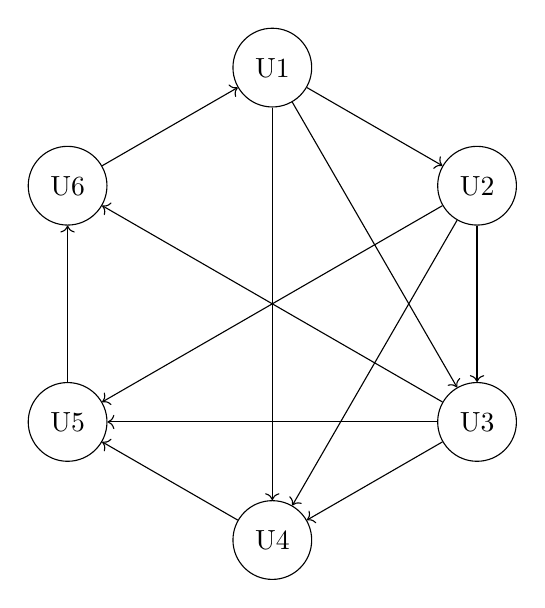
\begin{tikzpicture}[
    node distance=2.5cm,
    every node/.style={circle,draw,minimum size=1cm}
]
% Đặt các node theo hình lục giác đều
\node (U1) at (0,3) {U1};
\node (U2) at (2.6,1.5) {U2};
\node (U3) at (2.6,-1.5) {U3};
\node (U4) at (0,-3) {U4};
\node (U5) at (-2.6,-1.5) {U5};
\node (U6) at (-2.6,1.5) {U6};

% Vẽ các cạnh có hướng
\draw[->] (U1) -- (U2);
\draw[->] (U1) -- (U3);
\draw[->] (U1) -- (U4);
\draw[->] (U2) -- (U3);
\draw[->] (U2) -- (U4);
\draw[->] (U2) -- (U5);
\draw[->] (U3) -- (U4);
\draw[->] (U3) -- (U5);
\draw[->] (U3) -- (U6);
\draw[->] (U4) -- (U5);
\draw[->] (U5) -- (U6);
\draw[->] (U6) -- (U1);
\end{tikzpicture}
\end{center}

\subsubsection{Mật độ mạng có hướng}
\[ D = \frac{12}{6 \times 5} = 0.400 \]

\subsubsection{Các số đo trung tâm}
\paragraph{a. In/Out-Degree Centrality}
\begin{center}
\begin{tabular}{|c|c|c|c|c|}
\hline
\textbf{User} & \textbf{In-deg} & \textbf{Out-deg} & $C_{D,in}$ & $C_{D,out}$ \\
\hline
U1 & 1 & 3 & 0.200 & 0.600 \\
U2 & 1 & 3 & 0.200 & 0.600 \\
U3 & 2 & 3 & 0.400 & 0.600 \\
U4 & 3 & 1 & 0.600 & 0.200 \\
U5 & 3 & 1 & 0.600 & 0.200 \\
U6 & 2 & 1 & 0.400 & 0.200 \\
\hline
\end{tabular}
\end{center}

\paragraph{b. In/Out-Closeness Centrality}
\begin{itemize}
\item In-Closeness:
    \begin{align*}
    C_{in}(U1) &= 0.714 & C_{in}(U4) &= 0.357 \\
    C_{in}(U2) &= 0.625 & C_{in}(U5) &= 0.417 \\
    C_{in}(U3) &= 0.625 & C_{in}(U6) &= 0.500
    \end{align*}
\item Out-Closeness:
    \begin{align*}
    C_{out}(U1) &= 0.455 & C_{out}(U4) &= 0.625 \\
    C_{out}(U2) &= 0.385 & C_{out}(U5) &= 0.625 \\
    C_{out}(U3) &= 0.455 & C_{out}(U6) &= 0.625
    \end{align*}
\end{itemize}

\paragraph{c. Betweenness Centrality (chuẩn hóa)}
\begin{align*}
C_B(U1) &= 0.500 & C_B(U4) &= 0.033 \\
C_B(U2) &= 0.033 & C_B(U5) &= 0.250 \\
C_B(U3) &= 0.133 & C_B(U6) &= 0.500
\end{align*}

\subsubsection{Phân tích vai trò và tương tác}
\begin{itemize}
\item \textbf{Phân nhóm chức năng:}
    \begin{itemize}
    \item Nhóm tạo nội dung (U1, U2, U3):
        \begin{itemize}
        \item Out-degree cao (0.600)
        \item Chủ động trong tương tác
        \item Nguồn phát sinh thông tin
        \end{itemize}
    \item Nhóm tiếp nhận (U4, U5):
        \begin{itemize}
        \item In-degree cao (0.600)
        \item Thu thập và xử lý thông tin
        \item Điểm hội tụ thông tin
        \end{itemize}
    \item Nhóm trung gian (U6):
        \begin{itemize}
        \item Cân bằng in/out degree
        \item Betweenness cao (0.500)
        \item Điều phối luồng thông tin
        \end{itemize}
    \end{itemize}

\item \textbf{Đặc điểm tương tác:}
    \begin{itemize}
    \item Tương tác hai chiều giữa các nhóm
    \item Tồn tại chu trình tương tác hoàn chỉnh
    \item Phân bố tương tác không đồng đều
    \end{itemize}

\item \textbf{Hiệu quả mạng:}
    \begin{itemize}
    \item Ưu điểm:
        \begin{itemize}
        \item Thông tin được phân phối đa chiều
        \item Có nhiều kênh tương tác thay thế
        \item Tồn tại các node trung tâm điều phối
        \end{itemize}
    \item Hạn chế:
        \begin{itemize}
        \item Phụ thuộc vào hoạt động của node trung tâm
        \item Có thể xảy ra tình trạng thông tin dư thừa
        \item Khó kiểm soát chất lượng thông tin
        \end{itemize}
    \end{itemize}
\end{itemize}

\end{document}